\documentclass[12pt, a4paper]{article}
\usepackage{enumitem}
\usepackage{fancyvrb}
\usepackage{float}
\usepackage[left=2cm, right=2cm, top=2cm, bottom=2cm]{geometry}
\usepackage{graphicx}
\usepackage[colorlinks, urlcolor=blue]{hyperref}
\usepackage{xeCJK}

\renewcommand\arraystretch{1.1}
\setCJKmainfont[AutoFakeBold=1.5]{新細明體}
\setlength{\parindent}{0pt}

\title{
  \vspace{-1cm}
  Network Administration/System Administration\\
  (NTU CSIE, Spring 2024)\\
  Homework \#9
}
\author{\Large B12902110 呂承諺}

\begin{document}
  \maketitle
  \section{No more Frieren Stuff}
  \begin{enumerate}[label=(\alph*)]
    \item \textbf{Steps}
    \begin{enumerate}[label=(\arabic*)]
      \item Set IP address of the server.
      \begin{Verbatim}[frame=single]
$ sudo ip addr add 192.168.30.1/24 broadcast + dev ens4
      \end{Verbatim}

      \item Set IP address of the client.
      \begin{Verbatim}[frame=single]
$ sudo ip addr add 192.168.30.2/24 broadcast + dev ens4
      \end{Verbatim}

      \item On the server, start the \verb|nfs-server| service.
      \begin{Verbatim}[frame=single]
$ sudo systemctl enable --now nfs-server.service
      \end{Verbatim}

      \item On the client, add the following line to \verb|/etc/fstab|.
      \begin{Verbatim}[frame=single]
# /etc/fstab
192.168.30.1:/srv/nfs/share /mnt/nfs-share nfs defaults 0 0
      \end{Verbatim}

      \item On the client, mount the volume.
      \begin{Verbatim}[frame=single]
$ sudo mount -a
      \end{Verbatim}
    \end{enumerate}

    \textbf{Result}
    \begin{Verbatim}[frame=single]
$ mount | grep nfs
$ ls -alh /mnt/nfs-share
    \end{Verbatim}

    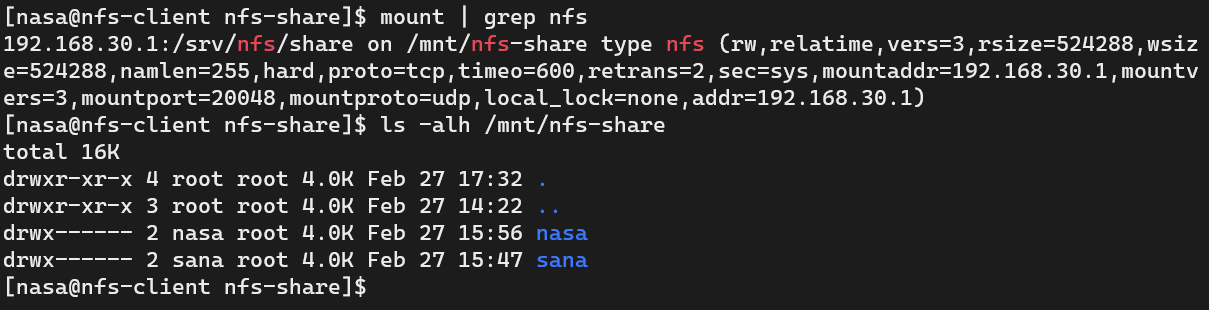
\includegraphics[width=0.95\textwidth]{1-a_result.png}

    \pagebreak
    \item \textbf{Steps}
    \begin{enumerate}[label=(\arabic*)]
      \item On the server, add \verb|no_root_squash| to the exports. Reload
      the configuration and restart the service.
      \begin{Verbatim}[frame=single]
  #/etc/exports
  /srv/nfs        192.168.30.2(rw,sync,fsid=0,no_root_squash)
  /srv/nfs/share  192.168.30.2(rw,sync,no_root_squash)
      \end{Verbatim}
      \begin{Verbatim}[frame=single]
$ sudo exportfs -arv
$ sudo systemctl restart nfs-server.service
      \end{Verbatim}
      \item On the client, create a file under \verb|/mnt/nfs-share|.
      \begin{Verbatim}[frame=single]
$ echo "# /mnt/nfs-share/file1.txt" |
    sudo tee /mnt/nfs-share/file1.txt
      \end{Verbatim}
    \end{enumerate}

    \textbf{Result}
    \begin{Verbatim}[frame=single]
$ ls -alh /srv/nfs/share
    \end{Verbatim}

    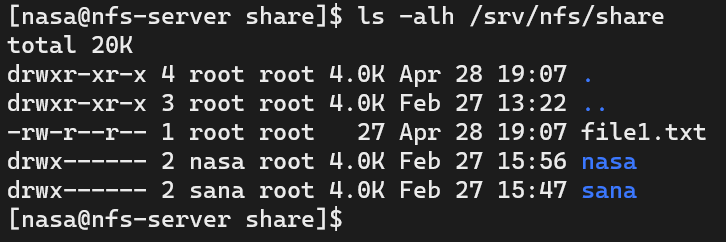
\includegraphics[width=0.5\textwidth]{1-b_result.png}

    \item \textbf{Steps}

    On the server, create \verb|/srv/nfs/share/asan| and modify the permissions.
    \begin{Verbatim}[frame=single]
$ sudo mkdir /srv/nfs/share/asan
$ sudo chown asan /srv/nfs/share/asan
$ sudo chmod 700 /srv/nfs/share/asan
    \end{Verbatim}

    \textbf{Result}
    \begin{Verbatim}[frame=single]
$ ls -alh /srv/nfs/share
    \end{Verbatim}

    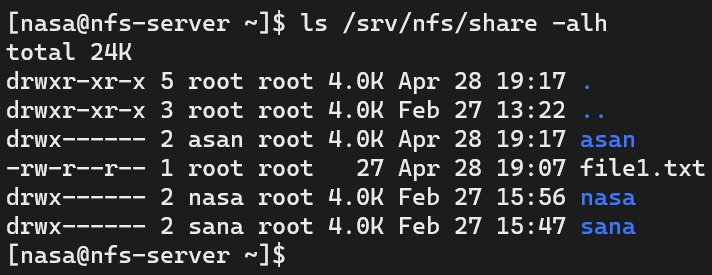
\includegraphics[width=0.5\textwidth]{1-c_result.png}
  \end{enumerate}

  \textbf{References}
  \begin{itemize}
    \item \href{https://wiki.archlinux.org/title/Network_configuration}{Network configuration - ArchWiki}
    \item \href{https://wiki.archlinux.org/title/NFS}{NFS - ArchWiki}
    \item \href{https://linux.die.net/man/5/nfs}{nfs(5) - Linux man page}
    \item \href{https://stackoverflow.com/questions/84882/sudo-echo-something-etc-privilegedfile-doesnt-work}{bash - sudo echo "something" >> /etc/privilegedFile doesn't work - Stack Overflow}
  \end{itemize}

  \pagebreak
  \section{Naughty Friend, Sana}
  \begin{enumerate}[label=(\alph*)]
    \item In the AUTH\_SYS authentication method, the user is authenticated at the
    the client. The client is responsible for telling the server the UID and GID.
    The server trusts and uses the UID and GID that the client provides.
    On the server, file permissions and ownership are kept just like any local user.
    \item \textbf{Steps}
    \begin{enumerate}[label=(\arabic*)]
      \item On both the server and the client, run \verb|getent passwd sana|.
      \begin{Verbatim}[frame=single]
[nasa@nfs-server ~]$ getent passwd asan
asan:x:1002:1002::/home/asan:/usr/bin/bash
      \end{Verbatim}
      \begin{Verbatim}[frame=single]
[nasa@nfs-client ~]$ getent passwd asan
asan:x:1010:1002::/home/asan:/usr/bin/bash
      \end{Verbatim}

      We discover that the UID doesn't match. It's 1002 on the server and 1010 on the client.

      \item Change asan's UID on the client to 1002.
      \begin{Verbatim}[frame=single]
$ sudo usermod -u 1002 asan
      \end{Verbatim}
    \end{enumerate}
    \textbf{Result}

    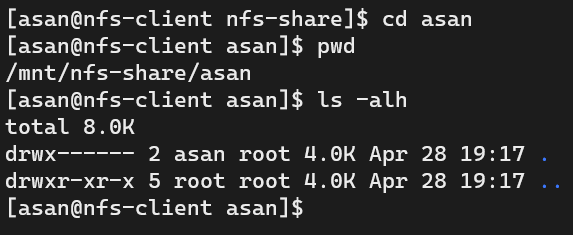
\includegraphics[width=0.6\textwidth]{2-b_result.png}
  \end{enumerate}

  \textbf{References}
  \begin{itemize}
    \item \href{https://access.redhat.com/documentation/en-us/red_hat_enterprise_linux/6/html/storage_administration_guide/s1-nfs-security#s3-nfs-security-hosts-nonnfsv4}{9.8. Securing NFS Red Hat Enterprise Linux 6 | Red Hat Customer Portal}
    \item \href{https://www.ibm.com/docs/en/aix/7.1?topic=management-nfs-v4-host-authentication}{NFS V4 host authentication}
  \end{itemize}

  \pagebreak
  \section{Nasa Finds krb5}
  \begin{enumerate}[label=(\alph*)]
    \item RPCSEC\_GSS uses the Kerberos protocol for authenticating users. It's based on
    symmetric-key cryptography, authentication servers, tickets and messages to provide
    mutual authentication over the Internet. Dedicated servers are responsible for
    authenticating users and issuing authorizations, so the previous trick would not
    work.

    \item \textbf{Steps}
    \begin{enumerate}[label=(\arabic*)]
      \item Install the \verb|chrony| package on both the server and client for time
      synchronization. Then start the \verb|chronyd| service.
      \begin{Verbatim}[frame=single]
$ sudo pacman -S chrony
$ sudo systemctl enable --now chronyd
      \end{Verbatim}
      \item Install the \verb|krb5| package on both the server and client.
      \begin{Verbatim}[frame=single]
$ sudo pacman -S krb5
      \end{Verbatim}
      \item Edit \verb|/etc/krb5.conf| on both the server and client to the following.
      \begin{Verbatim}[frame=single]
#/etc/krb5.conf
[libdefaults]
        default_realm = NASA.CSIE.NTU

[realms]
# use "kdc = ..." if realm admins haven't put SRV records into DNS
        NASA.CSIE.NTU = {
                admin_server = 192.168.30.1
                kdc = 192.168.30.1
        }
[domain_realm]
        nfs-server = NASA.CSIE.NTU
        nfs-client = NASA.CSIE.NTU
[logging]
        kdc = CONSOLE
      \end{Verbatim}
      \item Run the following commands on the server.
      \begin{Verbatim}[frame=single]
$ sudo kdb5_util create -s
$ sudo systemctl enable --now krb5-kdc.service krb5-kadmind.service
$ sudo kadmin.local
kadmin.local: addprinc nasa
kadmin.local: addprinc asan
kadmin.local: addprinc sana
kadmin.local: addprinc -randkey host/nfs-server
kadmin.local: ktadd -k kbclient.keytab host/nfs-server
kadmin.local: addprinc -randkey nfs/nfs-server
kadmin.local: ktadd -k kbclient.keytab nfs/nfs-serve
kadmin.local: addprinc -randkey host/nfs-client
kadmin.local: ktadd -k kbclient.keytab host/nfs-server
kadmin.local: quit
$ sudo scp kbclient.keytab nasa@192.168.30.2:~
$ sudo install -b -o root -g root -m 600 kbclient.keytab \
    /etc/krb5.keytab
      \end{Verbatim}

      \item Run the following commands on the client.
      \begin{Verbatim}[frame=single, fontsize=\footnotesize]
$ sudo install -b -o root -g root -m 600 kbclient.keytab \
    /etc/krb5.keytab
$ kinit
$ klist
Ticket cache: FILE:/tmp/krb5cc_1000
Default principal: nasa@NASA.CSIE.NTU

Valid starting     Expires            Service principal
04/28/24 12:50:03  04/29/24 12:50:03  krbtgt/NASA.CSIE.NTU@NASA.CSIE.NTU
      \end{Verbatim}

      \item Edit \verb|/etc/exports| on the server and add \verb|sec=krb5|, and then
      run \verb|exportfs -arv|.
      \begin{Verbatim}[frame=single]
# /etc/exports
/srv/nfs        192.168.30.2(rw,sync,fsid=0,no_root_squash,sec=krb5)
/srv/nfs/share  192.168.30.2(rw,sync,no_root_squash,sec=krb5)
      \end{Verbatim}
      \begin{Verbatim}[frame=single]
$ sudo exportfs -arv
      \end{Verbatim}
    \end{enumerate}
    \item \textbf{Result}

    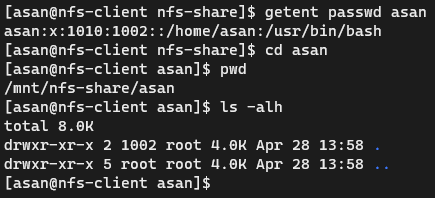
\includegraphics[width=0.7\textwidth]{3-c_result.png}
  \end{enumerate}

  \textbf{References}
  \begin{itemize}
    \item \href{https://en.wikipedia.org/wiki/Kerberos_(protocol)}{Kerberos (protocol) - Wikipedia}
    \item \href{https://access.redhat.com/documentation/zh-tw/red_hat_enterprise_linux/6/html/storage_administration_guide/s1-nfs-client-config-options}{9.5. Common NFS Mount Options Red Hat Enterprise Linux 6 | Red Hat Customer Portal}
    \item \href{https://wiki.archlinux.org/title/Kerberos}{Kerberos - ArchWiki}
    \item \href{https://unix.stackexchange.com/questions/134577/get-a-kerberos-service-ticket-from-the-command-line}{Get a Kerberos service ticket from the command line - Unix \& Linux Stack Exchange}
    \item \href{https://bbs.archlinux.org/viewtopic.php?id=272600}{NFS \& Kerberos not working: export does not exist / Networking, Server, and Protection / Arch Linux Forums}
    \item \href{https://bbs.archlinux.org/viewtopic.php?id=200165}{[SOLVED] Can't mount nfs share / Networking, Server, and Protection / Arch Linux Forums}
    \item \href{https://bbs.archlinux.org/viewtopic.php?id=289640}{Access denied while mounting nfsv4 with kerberos / Networking, Server, and Protection / Arch Linux Forums}
  \end{itemize}
\end{document}
